\documentclass[aspectratio=169,11pt]{beamer}
\usetheme{Madrid}
\usepackage{microtype,mathtools,amsmath,amssymb,bm,tikz}
\usetikzlibrary{arrows.meta,calc,positioning,decorations.pathreplacing}
\usepackage{pdfpages}

\setbeamersize{text margin left=10mm,text margin right=10mm}

% Macros
\newcommand{\R}{\mathbb{R}}
\newcommand{\grad}{\nabla}
\newcommand{\hess}{\nabla^2}
\newcommand{\vx}{\bm{x}}
\newcommand{\vtheta}{\bm{\theta}}
\newcommand{\vy}{\bm{y}}
\newcommand{\vg}{\bm{g}}
\newcommand{\vv}{\bm{v}}
\newcommand{\E}{\mathbb{E}}
\newcommand{\mX}{\bm{X}}
\newcommand{\MSE}{\text{MSE}}
\newcommand{\argmin}{\text{argmin}}

% Pop quiz counter
\newcounter{popquiz}

\title{Gradient Descent: The Foundation of ML Optimization}
\subtitle{From Taylor Series to Modern Deep Learning}
\author{Nipun Batra and Teaching Staff}
\institute{IIT Gandhinagar}
\date{\today}

\begin{document}

\maketitle

\begin{frame}{Outline}
\tableofcontents
\end{frame}

\section{Mathematical Foundations}

\begin{frame}{The Core ML Problem}
\begin{center}
\Large
\[\min_{\vtheta} f(\vtheta)\]
\end{center}

\pause
\textbf{Examples everywhere:}
\begin{itemize}
\item Linear regression: $\min (y - \mX\vtheta)^2$
\item Neural networks: $\min$ classification/regression loss
\item Logistic regression: $\min$ cross-entropy loss
\end{itemize}

\pause
\textbf{Challenge:} Most ML problems have no closed-form solution
\end{frame}

\begin{frame}{Geometric Intuition: Climbing Mountains}
\textbf{Imagine hiking in fog to reach the valley:}

\begin{itemize}
\item Feel slope beneath your feet
\item \textbf{Strategy:} Step in steepest downhill direction
\item \textbf{Gradient} = steepest \textcolor{red}{uphill}
\item \textbf{Negative gradient} = steepest \textcolor{blue}{downhill}
\end{itemize}

\pause
\begin{center}
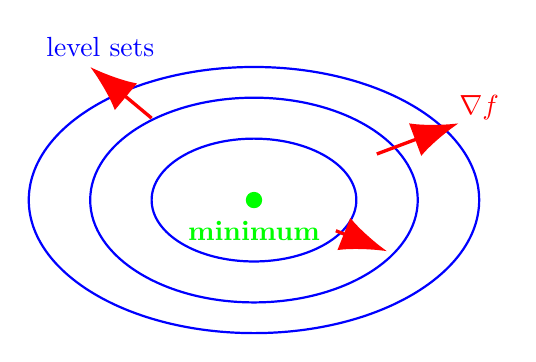
\begin{tikzpicture}[scale=1.3]
% Level sets (ellipses)
\draw[blue, thick] (0,0) ellipse (2.2 and 1.3);
\draw[blue, thick] (0,0) ellipse (1.6 and 1);
\draw[blue, thick] (0,0) ellipse (1 and 0.6);

% Gradient arrows (red, perpendicular to contours)
\draw[-{Latex[scale=2]}, red, very thick] (1.2,0.45) -- (2,0.75);
\draw[-{Latex[scale=2]}, red, very thick] (-1,0.8) -- (-1.6,1.3);
\draw[-{Latex[scale=2]}, red, very thick] (0.8,-0.3) -- (1.3,-0.5);

% Minimum point
\fill[green] (0,0) circle (0.08);
\node[green] at (0,-0.3) {\textbf{minimum}};

% Labels
\node[blue] at (-1.5,1.5) {level sets};
\node[red] at (2.2,0.9) {$\grad f$};
\end{tikzpicture}
\end{center}
\end{frame}

\begin{frame}{Think!}
\begin{center}
\Large \textbf{Think!}
\end{center}

Why does following $-\grad f$ lead us toward the minimum?

\pause
\vspace{1cm}
\textit{(Solution in Appendix)}
\end{frame}

\section{Taylor Series: The Mathematical Foundation}

\begin{frame}{Why Taylor Series?}
\textbf{Key insight:} If we can't solve $\min f(\vx)$ exactly, approximate $f(\vx)$ locally!

\pause
\textbf{Univariate Taylor expansion:}
\begin{center}
\Large
\[f(x) \approx f(x_0) + f'(x_0)(x-x_0) + \frac{1}{2}f''(x_0)(x-x_0)^2\]
\end{center}

\pause
\begin{itemize}
\item \textbf{Zero-order:} $f(x) \approx f(x_0)$ (constant)
\item \textbf{First-order:} adds linear term (tangent)
\item \textbf{Second-order:} adds quadratic curvature
\end{itemize}
\end{frame}

\begin{frame}{Visual: Tangent Line Approximation}
\begin{center}
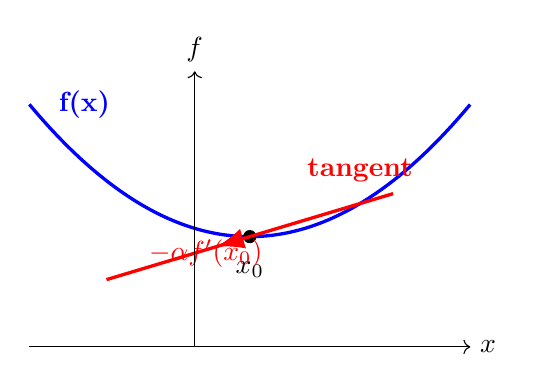
\begin{tikzpicture}[scale=1.4]
% Original function (blue curve)
\draw[blue, very thick, domain=-1.5:2.5, samples=100] 
  plot (\x, {0.3*(\x-0.5)*(\x-0.5) + 1});

% Point of tangency
\fill[black] (0.5,1) circle (0.06);
\node at (0.5,0.7) {$x_0$};

% Tangent line (red)
\draw[red, very thick, domain=-0.8:1.8] 
  plot (\x, {0.3*(\x-0.5) + 1});

% Step direction
\draw[-{Latex[scale=1.5]}, red, thick] (0.5,1) -- (0.2,0.91);
\node[red] at (0.1,0.85) {$-\alpha f'(x_0)$};

% Labels
\node[blue] at (-1,2.2) {\textbf{f(x)}};
\node[red] at (1.5,1.6) {\textbf{tangent}};

% Axes
\draw[->] (-1.5,0) -- (2.5,0) node[right] {$x$};
\draw[->] (0,0) -- (0,2.5) node[above] {$f$};
\end{tikzpicture}
\end{center}
\end{frame}

\begin{frame}{Visual: Adding Quadratic Term}
\begin{center}
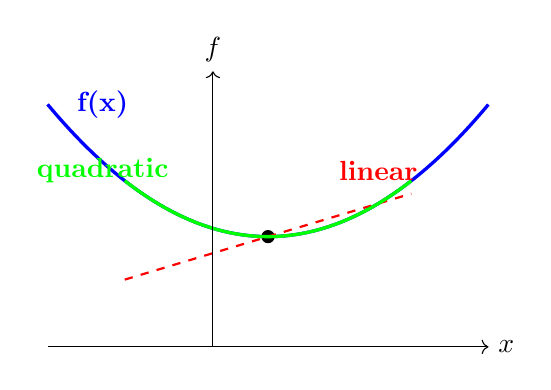
\begin{tikzpicture}[scale=1.4]
% Original function (blue curve)
\draw[blue, very thick, domain=-1.5:2.5, samples=100] 
  plot (\x, {0.3*(\x-0.5)*(\x-0.5) + 1});

% Point of tangency
\fill[black] (0.5,1) circle (0.06);

% Tangent line (red, dashed)
\draw[red, thick, dashed, domain=-0.8:1.8] 
  plot (\x, {0.3*(\x-0.5) + 1});

% Quadratic approximation (green)
\draw[green, very thick, domain=-0.8:1.8, samples=50] 
  plot (\x, {0.3*(\x-0.5)*(\x-0.5) + 1});

% Labels
\node[blue] at (-1,2.2) {\textbf{f(x)}};
\node[red] at (1.5,1.6) {\textbf{linear}};
\node[green] at (-1,1.6) {\textbf{quadratic}};

% Axes
\draw[->] (-1.5,0) -- (2.5,0) node[right] {$x$};
\draw[->] (0,0) -- (0,2.5) node[above] {$f$};
\end{tikzpicture}
\end{center}

\textbf{Key insight:} Higher-order terms give better approximations!
\end{frame}

\begin{frame}{Concrete Example: $f(x) = \cos(x)$ at $x_0 = 0$}
\begin{align}
f(0) &= \cos(0) = 1\\
f'(0) &= -\sin(0) = 0\\
f''(0) &= -\cos(0) = -1\\
f'''(0) &= \sin(0) = 0\\
f^{(4)}(0) &= \cos(0) = 1
\end{align}

\pause
\textbf{Taylor approximations:}
\begin{align}
\text{0th order:} \quad &f(x) \approx 1\\
\text{2nd order:} \quad &f(x) \approx 1 - \frac{x^2}{2}\\
\text{4th order:} \quad &f(x) \approx 1 - \frac{x^2}{2} + \frac{x^4}{24}
\end{align}
\end{frame}

\begin{frame}{Multivariate Taylor Series}
\begin{center}
\Large
\[f(\vx) \approx f(\vx_0) + \grad f(\vx_0)^T \Delta\vx + \frac{1}{2}\Delta\vx^T \hess f(\vx_0) \Delta\vx\]
\end{center}

\pause
where $\Delta\vx = \vx - \vx_0$

\pause
\begin{center}
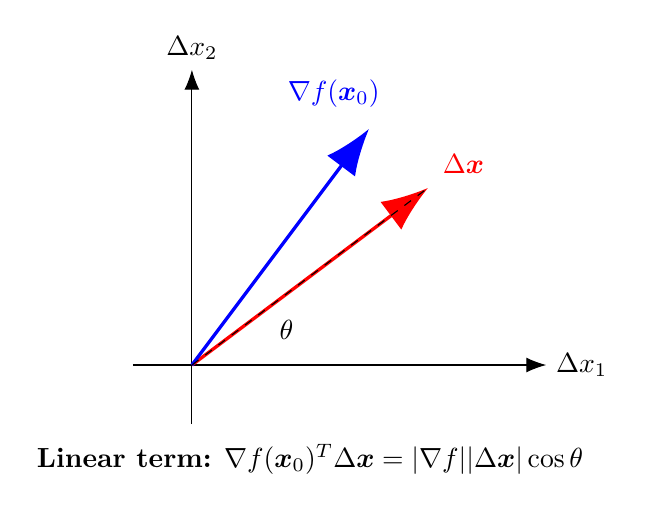
\begin{tikzpicture}[scale=1.5]
% Draw coordinate system
\draw[-{Latex[scale=1.5]}] (-0.5,0) -- (3,0) node[right] {$\Delta x_1$};
\draw[-{Latex[scale=1.5]}] (0,-0.5) -- (0,2.5) node[above] {$\Delta x_2$};

% Draw delta x vector
\draw[-{Latex[scale=2]}, red, very thick] (0,0) -- (2,1.5);
\node[red] at (2.3,1.7) {$\Delta\vx$};

% Draw gradient vector
\draw[-{Latex[scale=2]}, blue, very thick] (0,0) -- (1.5,2);
\node[blue] at (1.2,2.3) {$\grad f(\vx_0)$};

% Show dot product angle
\draw[dashed] (0,0) -- (1.33,1) -- (2,1.5);
\node at (0.8,0.3) {$\theta$};

\node at (1,-0.8) {\textbf{Linear term:} $\grad f(\vx_0)^T \Delta\vx = |\grad f||\Delta\vx|\cos\theta$};
\end{tikzpicture}
\end{center}
\end{frame}

\begin{frame}{Visual: Multivariate Case with Level Sets}
\begin{center}
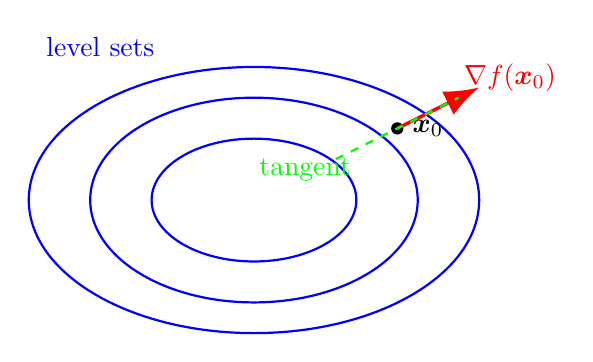
\begin{tikzpicture}[scale=1.3]
% Level sets
\draw[blue, thick] (0,0) ellipse (2.2 and 1.3);
\draw[blue, thick] (0,0) ellipse (1.6 and 1);
\draw[blue, thick] (0,0) ellipse (1 and 0.6);

% Point x0
\fill[black] (1.4,0.7) circle (0.06);
\node at (1.7,0.7) {$\vx_0$};

% Gradient vector (red)
\draw[-{Latex[scale=1.5]}, red, very thick] (1.4,0.7) -- (2.2,1.1);
\node[red] at (2.5,1.2) {$\grad f(\vx_0)$};

% Tangent plane indication
\draw[green, thick, dashed] (0.8,0.4) -- (2.0,1.0);
\node[green] at (0.5,0.3) {tangent};

\node[blue] at (-1.5,1.5) {level sets};
\end{tikzpicture}
\end{center}

\textbf{Key:} Gradient $\perp$ level sets, tangent plane $\perp$ gradient
\end{frame}

\section{Gradient Descent Algorithm}

\begin{frame}{From Taylor Series to Gradient Descent}
\textbf{Goal:} Find $\Delta\vx$ such that $f(\vx_0 + \Delta\vx) < f(\vx_0)$

\pause
\textbf{Using first-order Taylor approximation:}
\[f(\vx_0 + \Delta\vx) \approx f(\vx_0) + \grad f(\vx_0)^T \Delta\vx\]

\pause
\textbf{To minimize, we need:} $\grad f(\vx_0)^T \Delta\vx < 0$

\pause
\textbf{Vector geometry insight:} For vectors $\bm{a}$, $\bm{b}$: $\bm{a}^T\bm{b} = |\bm{a}||\bm{b}|\cos(\theta)$

Minimum when $\cos(\theta) = -1$ (opposite directions!)

\pause
\textbf{Optimal choice:} $\Delta\vx = -\alpha \grad f(\vx_0)$ where $\alpha > 0$

\pause
\begin{center}
\alert{\boxed{\vx_{\text{new}} = \vx_{\text{old}} - \alpha \grad f(\vx_{\text{old}})}}
\end{center}
\end{frame}

\begin{frame}{The Gradient Descent Algorithm}
\begin{center}
\alert{\boxed{\vtheta_{t+1} = \vtheta_t - \alpha \grad f(\vtheta_t)}}
\end{center}

\pause
\textbf{Algorithm:}
\begin{enumerate}
\item \textbf{Initialize:} $\vtheta_0$ (random or educated guess)
\item \textbf{For} $t = 0, 1, 2, \ldots$ until convergence:
\begin{itemize}
\item Compute gradient: $\vg_t = \grad f(\vtheta_t)$
\item Update parameters: $\vtheta_{t+1} = \vtheta_t - \alpha \vg_t$
\item Check convergence: $|\vg_t| < \epsilon$
\end{itemize}
\end{enumerate}

\pause
\textbf{Key properties:}
\begin{itemize}
\item First-order method (uses gradients, not Hessians)
\item Greedy local search
\item Guaranteed convergence for convex functions
\end{itemize}
\end{frame}

\section{Gradient Descent for Linear Regression}

\begin{frame}{Linear Regression Problem}
\textbf{Learn:} $y = \theta_0 + \theta_1 x$ from data

\begin{center}
\begin{tabular}{|c|c|}
\hline
\textbf{x} & \textbf{y} \\
\hline
1 & 1 \\
2 & 2 \\
3 & 3 \\
\hline
\end{tabular}
\end{center}

\pause
\textbf{Cost Function (Mean Squared Error):}
\[\MSE(\theta_0, \theta_1) = \frac{1}{n}\sum_{i=1}^n (y_i - \hat{y}_i)^2 = \frac{1}{n}\sum_{i=1}^n (y_i - \theta_0 - \theta_1 x_i)^2\]

\pause
\textbf{Goal:} $(\theta_0^*, \theta_1^*) = \argmin_{\theta_0, \theta_1} \MSE(\theta_0, \theta_1)$
\end{frame}

\begin{frame}{Computing Gradients for Linear Regression}
\textbf{We need:} $\grad \MSE = \begin{bmatrix} \frac{\partial \MSE}{\partial \theta_0} \\ \frac{\partial \MSE}{\partial \theta_1} \end{bmatrix}$

\pause
\textbf{Partial derivatives:}
\begin{align}
\frac{\partial \MSE}{\partial \theta_0} &= \frac{2}{n}\sum_{i=1}^n (y_i - \theta_0 - \theta_1 x_i)(-1) = -\frac{2}{n}\sum_{i=1}^n \epsilon_i\\
\frac{\partial \MSE}{\partial \theta_1} &= \frac{2}{n}\sum_{i=1}^n (y_i - \theta_0 - \theta_1 x_i)(-x_i) = -\frac{2}{n}\sum_{i=1}^n \epsilon_i x_i
\end{align}

where $\epsilon_i = y_i - \hat{y}_i$ is the residual.

\pause
\textbf{Matrix form:} $\grad \MSE(\vtheta) = \frac{2}{n}\mX^T(\mX\vtheta - \vy)$
\end{frame}

\begin{frame}{Step-by-Step Example}
\textbf{Initial:} $\theta_0 = 4$, $\theta_1 = 0$, $\alpha = 0.1$

\pause
\textbf{Iteration 1:}
\begin{itemize}
\item Predictions: $\hat{y}_1 = 4$, $\hat{y}_2 = 4$, $\hat{y}_3 = 4$
\item Errors: $\epsilon_1 = -3$, $\epsilon_2 = -2$, $\epsilon_3 = -1$
\item $\frac{\partial \MSE}{\partial \theta_0} = -\frac{2}{3}(-6) = 4$
\item $\frac{\partial \MSE}{\partial \theta_1} = -\frac{2}{3}(-10) = 6.67$
\item $\theta_0 = 4 - 0.1 \times 4 = 3.6$
\item $\theta_1 = 0 - 0.1 \times 6.67 = -0.67$
\end{itemize}

\pause
\textbf{New parameters:} $(\theta_0, \theta_1) = (3.6, -0.67)$
\end{frame}

\begin{frame}{Visual: GD Path on Loss Surface}
\begin{center}
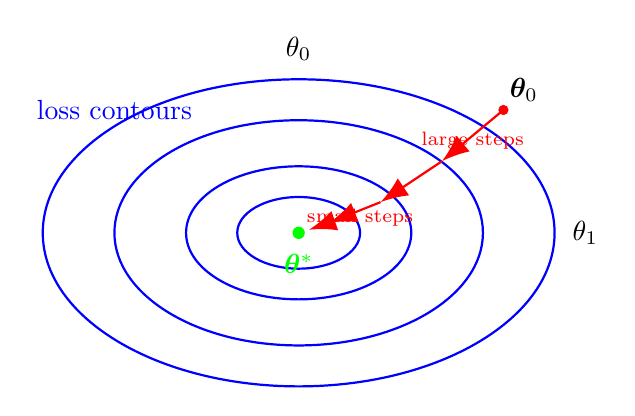
\begin{tikzpicture}[scale=1.3]
% Loss contours (elliptical)
\draw[blue, thick] (0,0) ellipse (2.5 and 1.5);
\draw[blue, thick] (0,0) ellipse (1.8 and 1.1);
\draw[blue, thick] (0,0) ellipse (1.1 and 0.65);
\draw[blue, thick] (0,0) ellipse (0.6 and 0.35);

% Minimum
\fill[green] (0,0) circle (0.06);
\node[green] at (0,-0.3) {$\vtheta^*$};

% GD path (red arrows showing steps)
\coordinate (p1) at (2,1.2);
\coordinate (p2) at (1.4,0.7);
\coordinate (p3) at (0.8,0.3);
\coordinate (p4) at (0.3,0.1);
\coordinate (p5) at (0.1,0.03);

\fill[red] (p1) circle (0.05);
\draw[-{Latex[scale=1.5]}, red, thick] (p1) -- (p2);
\draw[-{Latex[scale=1.5]}, red, thick] (p2) -- (p3);
\draw[-{Latex[scale=1.5]}, red, thick] (p3) -- (p4);
\draw[-{Latex[scale=1.5]}, red, thick] (p4) -- (p5);

\node at (2.2,1.4) {$\vtheta_0$};
\node[blue] at (-1.8,1.2) {loss contours};

% Axes labels
\node at (2.8,0) {$\theta_1$};
\node at (0,1.8) {$\theta_0$};

% Show step sizes getting smaller
\node[red] at (1.7,0.9) {\scriptsize large steps};
\node[red] at (0.6,0.15) {\scriptsize small steps};
\end{tikzpicture}
\end{center}

\textbf{Notice:} Algorithm takes larger steps when gradient is large!
\end{frame}

\section{Variants of Gradient Descent}

\begin{frame}{The Gradient Descent Family}
\textbf{Three main variants based on data usage per update:}

\begin{center}
\begin{tabular}{|l|c|c|c|}
\hline
\textbf{Method} & \textbf{Data per update} & \textbf{Updates per epoch} & \textbf{Convergence} \\
\hline
Batch GD & $n$ (all) & 1 & Smooth \\
SGD & 1 & $n$ & Noisy \\
Mini-batch GD & $b$ (batch size) & $n/b$ & Balanced \\
\hline
\end{tabular}
\end{center}

\pause
\textbf{Trade-offs:} Computational cost vs. convergence stability vs. memory

\pause
\textbf{Modern ML:} Mini-batch GD with batch sizes 32-256 is most common
\begin{itemize}
\item Good balance of stability and efficiency
\item Enables parallel computation (GPUs love batches!)
\end{itemize}
\end{frame}

\begin{frame}{Learning Rate Effects}
\begin{center}
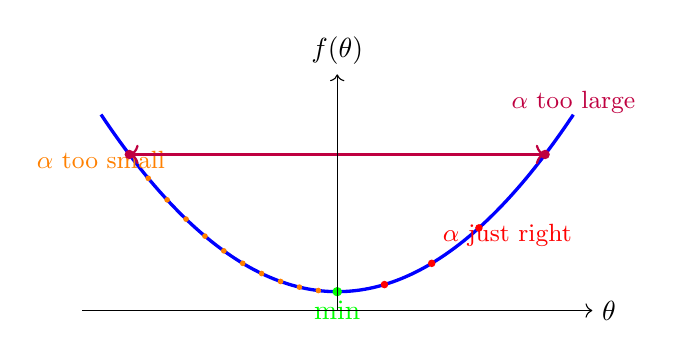
\begin{tikzpicture}[scale=1.2]
% Quadratic function
\draw[blue, very thick, domain=-2.5:2.5, samples=100] 
  plot (\x, {0.3*\x*\x + 0.2});

% Minimum
\fill[green] (0,0.2) circle (0.05);
\node[green] at (0,0) {min};

% Small alpha (many small steps)
\foreach \x in {-2,-1.8,-1.6,-1.4,-1.2,-1,-0.8,-0.6,-0.4,-0.2} {
  \fill[orange] (\x, {0.3*\x*\x + 0.2}) circle (0.03);
}
\node[orange] at (-2.5,1.6) {\small $\alpha$ too small};

% Good alpha (reasonable steps)  
\foreach \x in {1.5,1,0.5} {
  \fill[red] (\x, {0.3*\x*\x + 0.2}) circle (0.04);
}
\node[red] at (1.8,0.8) {\small $\alpha$ just right};

% Large alpha (overshoot)
\fill[purple] (2.2, {0.3*2.2*2.2 + 0.2}) circle (0.05);
\fill[purple] (-2.2, {0.3*2.2*2.2 + 0.2}) circle (0.05);
\draw[purple, thick, <->] (2.2, {0.3*2.2*2.2 + 0.2}) -- (-2.2, {0.3*2.2*2.2 + 0.2});
\node[purple] at (2.5,2.2) {\small $\alpha$ too large};

% Axes
\draw[->] (-2.7,0) -- (2.7,0) node[right] {$\theta$};
\draw[->] (0,0) -- (0,2.5) node[above] {$f(\theta)$};
\end{tikzpicture}
\end{center}
\end{frame}

\stepcounter{popquiz}
\begin{frame}{Pop Quiz \#\thepopquiz}
\begin{center}
\Large \textbf{Pop Quiz \#\thepopquiz}
\end{center}

For dataset with 1000 samples and batch size 50:
\begin{enumerate}
\item How many iterations per epoch for mini-batch GD?
\item If SGD takes 1000 epochs to converge, roughly how many epochs should mini-batch take?
\item Why might SGD be noisier than batch GD?
\end{enumerate}

\pause
\vspace{0.5cm}
\textit{(Solutions in Appendix)}
\end{frame}

\section{Mathematical Properties}

\begin{frame}{Convergence Rates for Convex Functions}
\textbf{$L$-smooth convex:} $\|\grad f(\vx) - \grad f(\vy)\| \leq L\|\vx-\vy\|$

With step size $\alpha \in (0, 1/L]$:
\[\alert{f(\vx_t) - f(\vx^*) \leq \frac{L\|\vx_0-\vx^*\|^2}{2t}}\]

\pause
\textbf{Rate:} $O(1/t)$ (sublinear)

\pause
\textbf{$\mu$-strongly convex + $L$-smooth:}
\[\alert{f(\vx_t) - f(\vx^*) \leq \left(1-\frac{\mu}{L}\right)^t (f(\vx_0) - f(\vx^*))}\]

\textbf{Rate:} Linear convergence! Condition number $\kappa = L/\mu$
\end{frame}

\begin{frame}{SGD as Unbiased Estimator}
\textbf{True gradient:} $\grad L(\vtheta) = \frac{1}{n}\sum_{i=1}^n \grad \ell(f(\vx_i;\vtheta),y_i)$

\textbf{SGD gradient estimate:} $\grad \tilde{L}(\vtheta) = \grad \ell(f(\vx;\vtheta),y)$, 
where $(\vx,y)$ is sampled uniformly from $\{(\vx_i,y_i)\}_{i=1}^n$

\pause
\textbf{Unbiased estimator property:}
\[\E[\grad \tilde{L}(\vtheta)] = \grad L(\vtheta)\]

\pause
\textbf{Proof sketch:}
\[\E[\grad \tilde{L}(\vtheta)] = \sum_{i=1}^n \frac{1}{n}\,\grad \ell(f(\vx_i;\vtheta),y_i) = \grad L(\vtheta)\]

\textbf{Implication:} Individual SGD steps might be ``wrong'', but average in correct direction!
\end{frame}

\begin{frame}{Why Unbiasedness Matters}
\textbf{Intuitive analogy:} Asking random people for directions
\begin{itemize}
\item Individual answers might be slightly off
\item But if no systematic bias, average direction is correct
\item SGD does the same with gradient estimates!
\end{itemize}

\pause
\textbf{The noise can be beneficial:}
\begin{itemize}
\item Helps escape local minima in non-convex problems
\item Provides implicit regularization
\item Enables online learning
\end{itemize}
\end{frame}

\section{Computational Complexity}

\begin{frame}{GD vs Normal Equation}
\textbf{For linear regression:}

\textbf{Normal equation:} $\hat{\vtheta} = (\mX^T\mX)^{-1}\mX^T\vy$
\begin{itemize}
\item Time complexity: $O(d^2n + d^3)$
\end{itemize}

\pause
\textbf{Gradient descent:} $\vtheta_{t+1} = \vtheta_t - \alpha \mX^T(\mX\vtheta_t - \vy)$
\begin{itemize}
\item Time complexity per iteration: $O(dn)$
\item Total: $O(T \cdot dn)$ for $T$ iterations
\end{itemize}

\pause
\textbf{When to use which?}
\begin{itemize}
\item Few features ($d < 1000$): Normal equation
\item Many features ($d > 10000$): Gradient descent
\item Non-linear models: Only gradient descent works
\end{itemize}
\end{frame}

\section{Advanced Topics and Extensions}

\begin{frame}{Beyond Basic Gradient Descent}
\textbf{Momentum:} $\vv_{t+1} = \beta \vv_t + (1-\beta)\vg_t$, $\vtheta_{t+1} = \vtheta_t - \alpha \vv_{t+1}$

\textbf{Adam:} Combines momentum + adaptive learning rates
\[\vtheta_{t+1} = \vtheta_t - \frac{\alpha}{\sqrt{\hat{\vv}_t} + \epsilon} \hat{\mathbf{m}}_t\]
Defaults: $\beta_1=0.9$, $\beta_2=0.999$, $\epsilon=10^{-8}$

\pause
\textbf{Why these improvements?}
\begin{itemize}
\item Handle different parameter scales automatically
\item Accelerate convergence in relevant directions
\item Reduce oscillations in narrow valleys
\end{itemize}
\end{frame}

\begin{frame}{Second-Order Methods}
\textbf{Newton's method:} $\vtheta_{t+1} = \vtheta_t - \alpha [\hess f(\vtheta_t)]^{-1} \grad f(\vtheta_t)$

\textbf{Gauss-Newton:} For least squares problems

\textbf{L-BFGS:} Quasi-Newton method (approximates Hessian)

\pause
\textbf{Trade-off:} Faster convergence vs. $O(d^3)$ cost per iteration

\pause
\textbf{Line search methods:} Adaptive step size via Armijo condition
\end{frame}

\begin{frame}{Gradient Descent in Deep Learning}
\textbf{Every modern deep learning framework uses GD variants!}

\textbf{Key extensions:}
\begin{itemize}
\item \textbf{Backpropagation:} Efficient gradient computation
\item \textbf{Automatic differentiation:} PyTorch/TensorFlow handle gradients
\item \textbf{GPU acceleration:} Parallel mini-batch gradients
\item \textbf{Mixed precision:} 16-bit + 32-bit arithmetic
\end{itemize}
\end{frame}

\section{Practical Considerations}

\begin{frame}{Learning Rate Selection}
\textbf{Common strategies:}
\begin{itemize}
\item Grid search: $\alpha \in \{0.001, 0.01, 0.1, 1.0\}$
\item Learning rate schedules: Start high, decay over time
\item Adaptive methods: Let algorithm adjust automatically
\item Learning rate finder: Gradually increase and watch loss
\end{itemize}

\pause
\textbf{Warning signs:}
\begin{itemize}
\item Loss exploding $\Rightarrow$ $\alpha$ too high
\item Very slow convergence $\Rightarrow$ $\alpha$ too low
\item Oscillating loss $\Rightarrow$ Try smaller $\alpha$ or momentum
\end{itemize}
\end{frame}

\begin{frame}{Other Practical Considerations}
\textbf{Feature scaling:} Standardize features: $(x - \mu)/\sigma$

\textbf{Convergence criteria:}
\begin{itemize}
\item Gradient magnitude: $\|\grad f(\vtheta)\| < \epsilon$
\item Function change: $|f(\vtheta_{t+1}) - f(\vtheta_t)| < \epsilon$
\item Maximum iterations: Simple upper bound
\end{itemize}

\pause
\textbf{Common pitfalls:}
\begin{itemize}
\item Poor initialization (use Xavier/He for neural networks)
\item Poor feature scaling (different parameter scales)
\item Not monitoring validation performance
\end{itemize}
\end{frame}

\begin{frame}{Think!}
\begin{center}
\Large \textbf{Think!}
\end{center}

For $L$-smooth function, why might $\alpha > 2/L$ cause divergence on a quadratic?

\pause
\vspace{1cm}
\textit{(Solution in Appendix)}
\end{frame}

\section{Summary and Key Takeaways}

\begin{frame}{What We've Learned}
\textbf{Core journey:}
\begin{itemize}
\item \textbf{Mathematical foundation:} Taylor series approximation
\item \textbf{Key insight:} Follow $-\grad f$ for steepest descent
\item \textbf{Algorithm:} $\vtheta_{t+1} = \vtheta_t - \alpha \grad f(\vtheta_t)$
\item \textbf{Variants:} Batch, SGD, mini-batch (use mini-batch!)
\item \textbf{Theory:} Convergence rates depend on function properties
\end{itemize}

\pause
\textbf{From theory to practice:}
\begin{itemize}
\item Tune learning rates carefully
\item Scale features properly
\item Monitor diagnostics
\item Consider advanced optimizers (Adam, momentum)
\end{itemize}

\pause
\begin{center}
\alert{\textbf{Gradient descent powers modern machine learning!}}
\end{center}
\end{frame}

% Include SGD theory PDF
\begin{frame}{Deep Dive: Stochastic Gradient Descent Theory}
\begin{center}
\textbf{For comprehensive mathematical analysis:}
\end{center}
\end{frame}

% Include SGD.pdf pages
\includepdf[pages=1-5,fitpaper]{../assets/SGD.pdf}

\appendix
\section{Appendix}

\begin{frame}{Think! Solutions}
\textbf{Think! 1:} Why does $-\grad f$ lead toward minimum?

The gradient $\grad f(\vx)$ points in direction of steepest \emph{ascent}. To \emph{descend} (minimize), we go in the opposite direction: $-\grad f(\vx)$.

\pause
\vspace{0.5cm}
\textbf{Think! 2:} Why might $\alpha > 2/L$ cause divergence?

For quadratic $f(x) = \frac{L}{2}x^2$, we have $f'(x) = Lx$. 
The update becomes: $x_{t+1} = x_t - \alpha L x_t = (1-\alpha L)x_t$. 

If $\alpha L > 2$, then $|1-\alpha L| > 1$, causing the sequence to diverge.
\end{frame}

\begin{frame}{Pop Quiz Solutions}
\textbf{Pop Quiz \#1:} For 1000 samples, batch size 50:
\begin{enumerate}
\item Mini-batch iterations per epoch: $1000/50 = 20$
\item If SGD takes 1000 epochs, mini-batch might take $\approx 50$ epochs (rough estimate)
\item SGD is noisier because it uses only 1 sample per update vs. all samples for batch GD
\end{enumerate}

\pause
\vspace{0.5cm}
\textbf{Additional insight:} The noise in SGD can actually help escape local minima in non-convex optimization problems!
\end{frame}

\begin{frame}{References \& Further Reading}
\textbf{Essential references:}
\begin{itemize}
\item Boyd \& Vandenberghe: \emph{Convex Optimization}
\item Nocedal \& Wright: \emph{Numerical Optimization}
\item Goodfellow et al.: \emph{Deep Learning}, Chapters 4 \& 8
\end{itemize}

\pause
\textbf{Interactive resources:}
\begin{itemize}
\item Gradient descent visualizations online
\item Implement from scratch in NumPy/PyTorch
\item Experiment with different learning rates
\end{itemize}

\pause
\vspace{0.5cm}
\begin{center}
\textbf{Next lecture:} Advanced Optimization Techniques\\
\textbf{Practice:} Implement GD for your favorite ML model!
\end{center}
\end{frame}

\end{document}